\documentclass[10pt,a4paper]{article}
\usepackage[utf8]{inputenc}
\usepackage{amsmath}
\usepackage{amsfonts}
\usepackage{amssymb}
\newcommand\tab[1][1cm]{\hspace*{#1}}
\usepackage{graphicx}
\usepackage{scrextend}
\usepackage{wrapfig}
\author{Konrad Cybulski}
\title{Using agent-based simulations to verify the predictions made by Santos, Santos, Pacheco.}
\begin{document}
\begin{titlepage}
    \begin{center}
        \vspace*{1cm}
        
        \LARGE
        \textbf{Using agent-based simulations to investigate rates of cooperation in small populations and verify the findings of Santos, Santos and Pacheco}
        
        \vspace{2cm}
        \Large
        
        \textbf{Konrad Cybulski}
        
        \vfill
        
        Final report for\\
        FIT1041 Research Project
        
        \vspace{0.8cm}
        
        
\includegraphics[width=0.4\textwidth]{monash_emblem.jpg}
        
        \large
        Faculty of Information Technology\\
        Monash University\\
        Australia\\
        24/10/2016
        
    \end{center}
\end{titlepage}

\begin{Large}

\end{Large}

\pagebreak
\tableofcontents
\pagebreak

\section{Abstract}
In order to understand our behaviour, our willingness and ability to cooperate with those around us, it is vital that we can create simulations to model the dynamics of populations and the interactions of agents within them.
It is also important to understand the way cooperation and defection evolve in both small and large populations.
The main research paper on which this project is based is “\textit{Social Norms of Cooperation in Small-Scale Societies}” by Santos, Santos, and Pacheco. 
In the paper a number of simulation parameters and methods are introduced and those specifications are replicated in this project in order to verify the results of the simulations performed in the paper.
\section{Introduction}
The primary aim of this project is to replicate the findings of Santos, Santos, and Pacheco which will allow further exploration into more detailed models of the prisoner’s dilemma game within populations. The paper outlines simulation parameters based on equations to model the process in which the prisoner’s dilemma game is played over time in a population. 
In order to allow for greater research to be done in this area based on the simulation developed to verify the mathematical model developed by Santos et al. it is necessary that the simulation can be recreated and tested under similar variables and constraints to verify their results.
\\

\begin{wrapfigure}{r}[6em]{0.6\linewidth}
  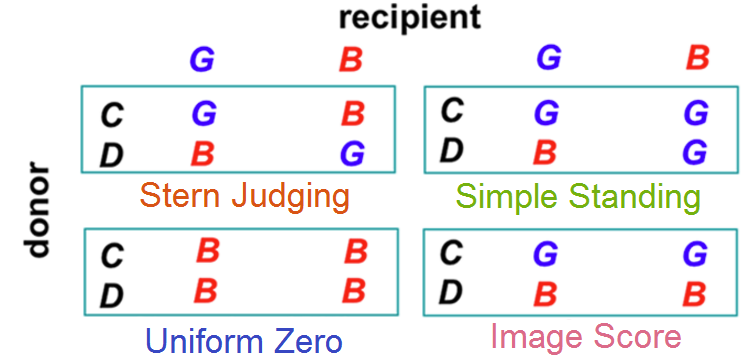
\includegraphics[width=\linewidth]{social_norms.PNG}
  \caption{Social norms \textit{Stern Judging}, \textit{Simple Standing}, \textit{Zero Uniform} and \textit{Image Score}.}
  \label{fig:Runtime1}
\end{wrapfigure}

The four social norms investigated in this verification include two norms leading to extremely low cooperation indexes and the only two leading to high rates of cooperation.
The social norms are defined as Stern Judging (high cooperation rate), Simple Standing (high cooperation rate), Image Score (low cooperation rate) and Uniform Zero (low cooperation rate).
Each social norm is defined as a way of assigning reputation to an agent after an interaction based on their action (Cooperation or Defection) and the reputation of the other agent (Good or Bad).

\section{Methodology}
The application developed was initially programmed in pure Python and based on the pseudocode provided by Santos, Santos, Pacheco in the supporting material of their paper.
In developing both the Python program, the focus initially was on optimization of the program due to the intractability of the algorithm as defined in the paper for large population sizes (\emph{Z}), large generation numbers (\emph{G}) and large numbers of runs (\emph{R}).
The total time complexity for any given simulation being O(\emph{$Z^{2} \cdot G\cdot R$}).
Utilising numpy $^{3}$ a number of scalar optimisations were able to increase the efficiency of the program in its Python implementation. 
The majority of the optimisation however was done by utilising Cython.
\\
The method of vectorizing the program took was aimed at parallelizing the stage at which one individual interacted with a number of other individuals in order to determine its average fitness over a number of interactions. 
All optimizations made at any point in the algorithm were tested to ensure complete correctness and verify the algorithm itself had been altered functionally in any way.
\subsection{Vectorization of the fitness function}
The fitness function, the function to determine the average fitness of an individual over the course of a series of prisoner's dilemma games with other individual in the population, was the aim of the optimization. 
The vectorization was required to compute a series of vectors in order to computer the payoff for a given agent X and update the reputations of X and a vector of other agents (the tournament vector).
The following computations were required:
\\
\\ 1. Vector of actions taken by a given agent X against each opposing individual in the tournament vector.
\\ 2. Vector of actions taken by each agent in the tournament vector.
\\ 3. Vector of the reputation of X after each interaction.
\\ 4. Vector of the reputation of each agent after each interaction with X. \\\\

The equations defining the actions of both agent X (\emph{$C_{x}$}) and each agent in the tournament vector (\emph{$C_{y}$}) are defined as:\\
$A_{i}$ = the vector of size two defining the possible actions of agent i against another agent Y, this vector contains the action if Y has reputation G and if Y has reputation B.\\
$(A_{i})_{G}$ = the action of agent X if the reputation of some agent Y is G (0 is defection, 1 is cooperation). \\
$(A_{i})_{B}$ = the action of agent X if the reputation of some agent Y is B (0 is defection, 1 is cooperation). \\
R = the reputations of the agents defined in the tournament vector (0 is B, 1 is G). \\
$R_{x}$ = the reputation of agent X (0 is B, 1 is G). 
\begin{center}
$\overrightarrow{C_{x}} = (A_{x})_{G} \cdot \overrightarrow{R} + (A_{x})_{B} \cdot (1 - \overrightarrow{R})$
\\
$\overrightarrow{C_{y}} = \overrightarrow{(A_{y})_{G}} \cdot \overrightarrow{R_{x}} + \overrightarrow{(A_{y})_{B}} \cdot (1 - \overrightarrow{R_{x}})$
\end{center}

The constraints of this vectorization however are such that for any given tournament vector there must be no duplicates.
Due to the parallel nature of the interactions, interactions are performed with incorrect or antiquated knowledge of the reputation of an agent who appears more than once.
In order to perform the fitness function correctly with duplicate agents in the tournament sample the algorithm must iterate through each agent.
Thus the vectorization requires that a given tournament sample must not contain duplicate agents.
\\\\
The parallelization of reputation update was done utilizing \emph{numpy} features.

\subsection{Analysis of optimization}
The optimizations made to increase the program's time complexity and execution time were measured utilizing \emph{Jupyter Notebook}.

%\pagebreak
\section{Results}
\begin{figure}[h!]
  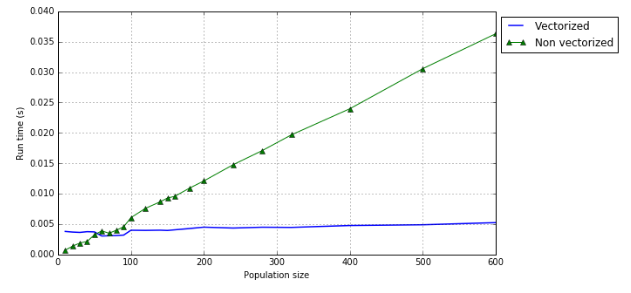
\includegraphics[width=\linewidth]{Vectorized_python_speedup.PNG}
  \caption{Run time of the fitness function for both pure Python implementation and vectorized Python implementation for $10 \leq \emph{Z} \leq 600$.}
  \label{fig:Runtime1}
\end{figure}

\begin{figure}[h!]
  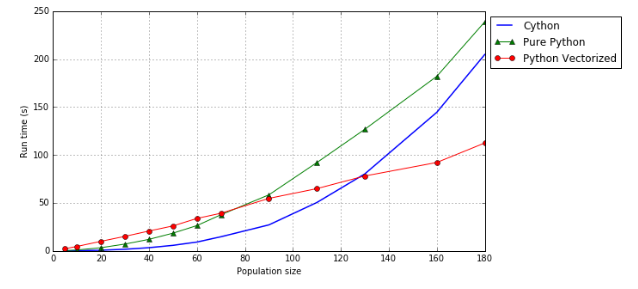
\includegraphics[width=\linewidth]{cython_python_vectorized_run_time.PNG}
  \caption{Run time of entire simulation for G=$3 \cdot 10^{2}$ and $5 \leq \emph{Z} \leq 180$ of pure Python, vectorized Python, and Cython versions of the simulation.}
  \label{fig:Runtime1}
\end{figure}

\begin{figure}[h!]
\begin{center}
  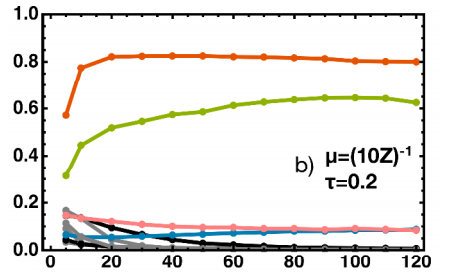
\includegraphics[width=28em]{SSP_Results.PNG}
  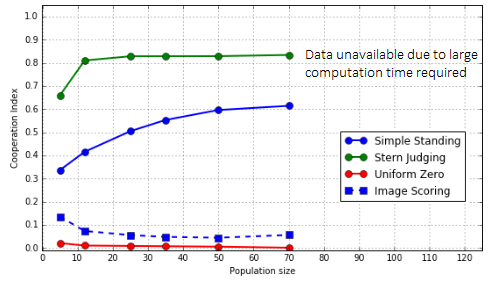
\includegraphics[width=27em]{simulation_results_cropped.PNG}
\end{center}
  \caption{Results of Santos Santos Pacheco$^{[2]}$ (Top) and the simulation specified in this report (Bottom) under parameters $\epsilon = 0.08, \chi = 0.01, \alpha = 0.01, \mu = (10 \cdot Z)^{-1}$.}
  \label{fig:SSPresults1}
\end{figure}
\pagebreak

\section{Discussion}

\subsection{Vectorization of the fitness function}
The pure Python vectorization of the simulation aimed to reduce the overall time complexity of the fitness function from O(\emph{Z}) to O(1).
While all vector operations performed may take up to O(N) time complexity at a lower level, due to the large overhead of Python function calls the vectorized function reduces the number of function calls from \emph{Z} to 1.
\\
The fitness function itself reduces to almost O(1) for values of $\emph{Z}$ within the testing range $(\emph{Z} \in [10, 600])$ (\textit{Figure 2}).
While the vectorized fitness function is slower than the non-vectorized function, for very large population sizes, it allows the simulation to be tractable and brings the total simulation time complexity to O(\emph{$Z \cdot G\cdot R$}).
\\
As evident in \textit{Figure 3}, the vectorized function performs much worse on smaller population sizes compared to both the pure Python and Cython programs, however past the mark of \emph{Z}=130, the vectorized function performs much faster with a greatly improved rate of increase.
This reduction in time complexity allows further work to be done on larger population sizes and to aid in the understanding of reputation and its effect on cooperation in population sizes of greater than 130.

\subsection{Verification of results}
Simulations were tested using $\epsilon = 0.08, \chi = 0.01, \alpha = 0.01, \mu = (10 \cdot Z)^{-1}, \tau = 1.0$, and contrasted against the data provided in the supporting material of Santos, Santos, Pachecho given $ 5 \leq \emph{Z} \leq 70.$
As shown in \textit{Figure 4}, the program produced results that closely reflect those of the paper. 
The four social norms investigated were Stern Judging, Simple Standing, Uniform Zero and Image Score
Each of the results was the average of R=100 runs and G=$3 \cdot 10^{5}$ generations. 
Thus the simulation produced verifies the results produced in the paper according to the simulation parameters detailed in the supporting material given the simulations performed and shown in this report.

\subsection{Further work}
With a simulation developed that is both fast for small population sizes and tractable for large populations, there is a platform for testing new models with relatively small changes to the simulation itself.
As shown in section 6 (\textit{Extension}) there lies little difficulty in implementing new functionality to test both different parameters and different processes by which we perform the simulation.
\\
Regarding large population sizes, there exists work that can be done regarding converting the vectorized Python simulation to a Cython or C/C++ program to improve the speed again.
Further improvements can be made to the program to increase the speed of the simulation including converting of the Cython program to pure C/C++ in addition to the vectorized simulation.
This adaptation will most likely further improve the run time of the simulation for small population sizes ($\emph{Z} \leq 130$) in a similar fashion to that shown in \textit{Figure 3}.
\\

\pagebreak
\section{Extension}
The method by which Santos, Santos and Pacheco incorporate private assessment errors of the reputation of any other agent in the simulation involves the use of a single variable $\chi$ which determines this error for all agents.
The error $\chi$ determines the probability that a given agent will wrongly assess the reputation of another agent in a given interaction.
The extension on this project aimed to investigate the effect of dynamic assessment errors and the delay of reputation information propagation on rates of cooperation.
The process by which this variable assessment error is incorporated into the simulation is outlined in \textit{Methodology (6.1)}
$ \\\\ $
While it is expected that the cooperation index for smaller population sizes will stay relatively constant for a given social norm in comparison to a constant private assessment error, for larger population sizes, this propagation delay may have a greater impact on the rate of cooperation.

$ $

\subsection{Methodology}
The likelihood of wrongly assessing the reputation of a given individual is defined as a function of the time since the last update of that individual's reputation.
In turn this process emulates the delay that exists between the creation of new information about an agent's reputation and when any other agent in the population comes into that knowledge.
The way that this is done, while maintaining the stochastic framework of the simulation itself, is by utilizing a function for the private assessment error for a given individual \textit{i} (denoted further as $\chi_{i}$) and keeping track only of the number of time steps (interactions, denoted as $\textit{t}_{i}$) since agent-\textit{i}'s reputation was \emph{changed}.
While we may update an agent's reputation after every interaction, $\textit{t}_{i}$ is only reset to 0 when $R_{i}$ has been changed to a value other than its current value.
\\
The private assessment error the function is defined as: \\
\begin{addmargin}[1em]{2em}
$\chi_{min}$ = the minimum private assessment error. \\
Z = the population size. \\
$R_{s}$ = the rate of information spread. 
\begin{addmargin}[2em]{1em}
For $R_{s} \in [0, 1]$, $R_{s}$ of value \textbf{\textit{a}} signifies that at each interaction every agent with knowledge of agent-\textit{i}'s reputation will give this information to another agent with probability \textbf{\textit{a}}. \\
For $R_{s} > 1$,  $R_{s}$ signifies that at each interaction every agent with knowledge of agent-\textit{i}'s reputation will give this information to $R_{s}$ other agents.
\end{addmargin}
\end{addmargin}
\begin{center}
$ \chi(t) = 1 - \chi_{min} - \dfrac{(1 + R_{s})^{t}}{Z},\tab \chi_{min} \leq \chi(t) \leq  1 - \chi_{min}$ \\
\end{center}

\subsection{Results}

\subsection{Discussion}

\subsection{Further work}


\pagebreak
\begin{thebibliography}{9}

\bibitem{1} 
Martin A. Novak, Karl Sigmund, (2005) 
\textit{Evolution of indirect reciprocity}. 
Nature.

\bibitem{2} 
Fernando P. Santos, Francisco C. Santos, Jorge M. Pacheco, (2016) 
\textit{Social Norms of Cooperation in Small-Scale Societies}. 
PLOS Computational Biology.

\bibitem{3} 
Numpy Developers, (2016) 
\textit{Numpy}. 
\\\texttt{http://www.numpy.org/}.

\bibitem{4} 
Continuum Analytics, Inc., (2016) 
\textit{Anaconda and Anaconda Accelerate}. 
\\\texttt{https://docs.continuum.io/}.

\bibitem{5} 
Hisashi Ohtsuki, Yoh Iwasa, (2005) 
\textit{The leading eight: Social norms that can maintain cooperation by indirect reciprocity}. 
Journal of Theoretical Biology.

\bibitem{6} 
Olof Leimar, Peter Hammerstein, (2001) 
\textit{Evolution of cooperation through indirect reciprocity}. 
Proceedings of the Royal Society B.

\end{thebibliography}
\end{document}